\documentclass[aspectratio=169]{beamer}

\usetheme{Madrid}
\usecolortheme{dolphin}
\usepackage{booktabs}
\usepackage{graphicx}
\usepackage{hyperref}
\usepackage{array}

\title[Mechanistic Model Merging]{Mechanistic Model Merging}
\subtitle{Plain-language overview, project plan, evidence so far, and current checkpoint}
\author{Gavin + Codex}
\date{May 20, 2026}

\begin{document}

\begin{frame}
  \titlepage
\end{frame}

\begin{frame}{One-Slide Summary}
  \begin{itemize}
    \item \textbf{Model merging} combines trained model weights or fine-tuning deltas into one model, often without the original training data.
    \item \textbf{Our project} asks why merging works or fails mechanistically, using the same discipline as the value-action project: prove the basis first, then interpret.
    \item \textbf{Current case} is a public Qwen2.5-1.5B merge where an abliterated TIES model loses harmful-refusal behavior while keeping benign behavior.
    \item \textbf{Main result today:} restoring a low-rank MLP activation-delta subspace over layers 12-24 repairs refusal behavior; strict manual audit makes \texttt{pca\_rank64} the strongest compressed baseline.
    \item \textbf{Next step:} harden the refusal evaluator, validate on held-out prompts, then compare SAE/transcoder features against PCA rank 64.
  \end{itemize}
\end{frame}

\section{Model Merging Basics}

\begin{frame}{What Is Model Merging?}
  A neural network is a large table of learned numbers, called \textbf{weights}.

  \vspace{0.35cm}
  Model merging means:
  \begin{itemize}
    \item start with two or more trained checkpoints;
    \item combine their weights, or the changes from a shared base model;
    \item produce one model that hopefully inherits useful behavior from each source.
  \end{itemize}

  \vspace{0.35cm}
  It is done \textbf{before inference}. It is not asking several models and voting.
\end{frame}

\begin{frame}{The Simplest Version}
  If two models start from the same base, a fine-tuned expert can be written as:

  \[
    \theta_{\text{expert}} = \theta_{\text{base}} + \Delta_{\text{task}}
  \]

  A simple merged model can be:

  \[
    \theta_{\text{merge}} =
    \theta_{\text{base}}
    + \alpha \Delta_{\text{math}}
    + \beta \Delta_{\text{code}}
    + \gamma \Delta_{\text{safety}}
  \]

  \vspace{0.2cm}
  Here, the deltas are task vectors: directions in weight space created by fine-tuning.
\end{frame}

\begin{frame}{Merging Is Not Concatenation}
  \begin{figure}
    \centering
    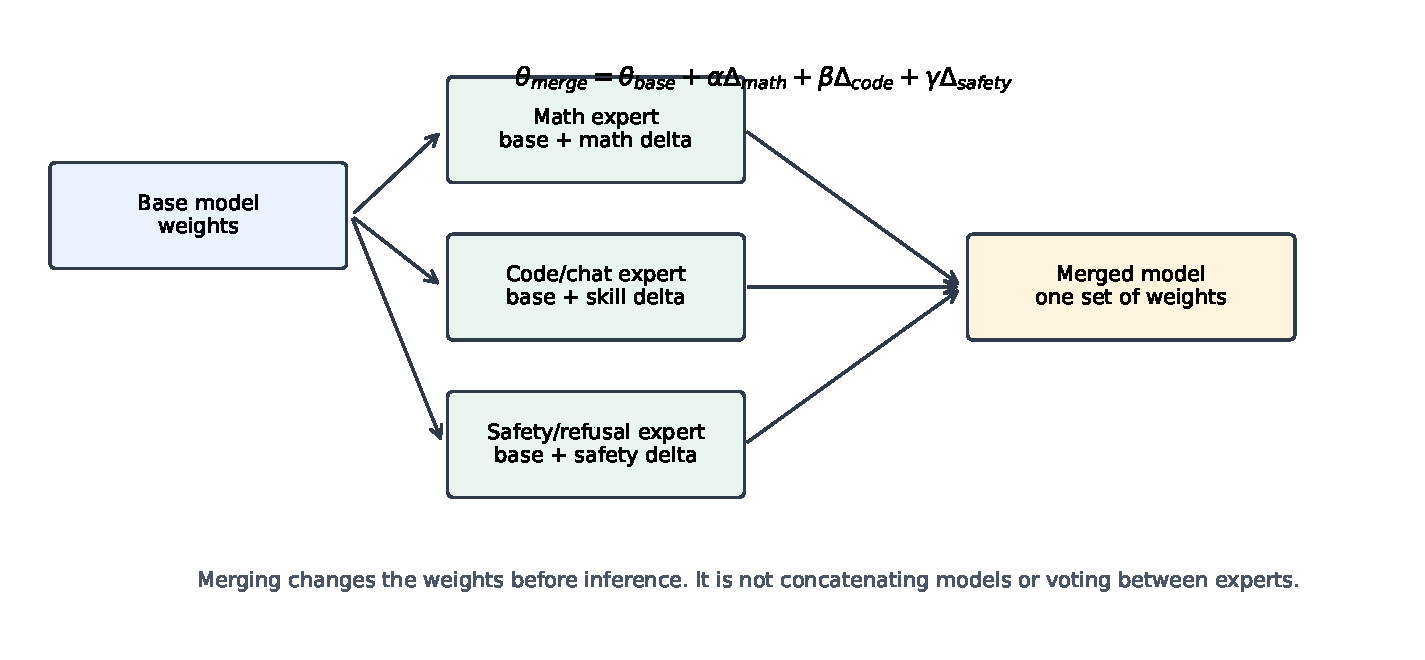
\includegraphics[width=0.92\linewidth]{figures/merge_concept.pdf}
  \end{figure}
\end{frame}

\begin{frame}{Why People Use It}
  Model merging is useful when:
  \begin{itemize}
    \item you have useful expert checkpoints but not the original training data;
    \item full joint training is too expensive;
    \item data cannot be shared because of privacy, license, or organization boundaries;
    \item you want one deployable model instead of many models at inference time;
    \item open-source communities want to combine math, code, chat, multilingual, or safety behavior.
  \end{itemize}

  \vspace{0.25cm}
  Important: the claim is usually not ``better than ideal full training.'' The claim is often ``better than what we can do with only checkpoints.''
\end{frame}

\begin{frame}{Why It Is Hard To Understand}
  Merging can fail even when each source model is good.

  \begin{itemize}
    \item Two models may solve tasks using incompatible internal coordinates.
    \item Deltas may point in conflicting directions.
    \item A behavior may need multiple components: detection, policy, wording, formatting, and termination.
    \item A merge may preserve a keyword but lose the full mechanism.
    \item Metrics can over-credit shallow behavior, such as starting with a refusal and then giving unsafe advice.
  \end{itemize}
\end{frame}

\begin{frame}{Related Work Anchors}
  \scriptsize
  \begin{tabular}{p{0.22\linewidth}p{0.36\linewidth}p{0.30\linewidth}}
    \toprule
    Work & What it does & Why it matters here \\
    \midrule
    McMahan et al., FedAvg, AISTATS 2017 & average client model updates & predecessor of checkpoint averaging \\
    Izmailov et al., SWA, UAI 2018 & average training checkpoints & averaging can find wider optima \\
    Garipov et al., Mode Connectivity, NeurIPS 2018 & low-loss paths between trained models & averaging works better when models are compatible \\
    Wortsman et al., Model Soups, ICML 2022 & average fine-tuned checkpoints & modern same-base merging result \\
    Ilharco et al., Task Arithmetic, ICLR 2023 & add/subtract task vectors & delta view of model editing \\
    Yadav et al., TIES-Merging, NeurIPS 2023 & trim and resolve sign conflicts & practical interference handling \\
    Yu et al., DARE, ICML 2024 & random delta dropping/rescaling & shows redundancy in deltas \\
    Goddard et al., MergeKit, arXiv 2024 & tooling for LLM merging & makes community merging practical \\
    \bottomrule
  \end{tabular}

  \vspace{0.15cm}
  \tiny Citation counts are in the local project proposal; this slide is the conceptual map.
\end{frame}

\section{Project Goal}

\begin{frame}{What We Want To Do}
  \textbf{Central question:}

  \vspace{0.15cm}
  When model merging works or fails, can we explain it in terms of identifiable mechanisms, features, modules, and causal pathways rather than only benchmark scores?

  \vspace{0.4cm}
  \textbf{Near-term target:}
  \begin{itemize}
    \item find a clean public-model merge failure;
    \item localize the missing behavior internally;
    \item repair it with causal interventions;
    \item then ask whether SAE/transcoder features explain more than raw activations, PCA, random projections, neurons, or module patching.
  \end{itemize}
\end{frame}

\begin{frame}{Project Pipeline}
  \begin{figure}
    \centering
    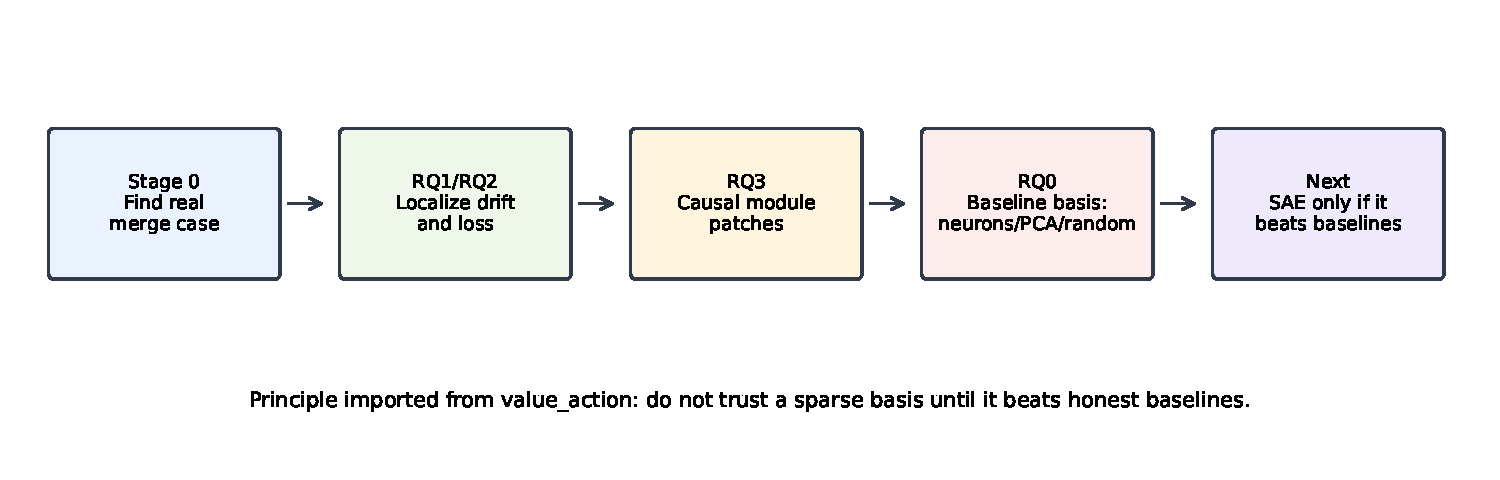
\includegraphics[width=0.94\linewidth]{figures/project_pipeline.pdf}
  \end{figure}
\end{frame}

\begin{frame}{Core Research Discipline}
  Borrowed from the value-action style:

  \begin{enumerate}
    \item Do not assume sparse features are meaningful because they look interpretable.
    \item First test raw baselines: modules, activations, neurons, PCA, random projections, deltas.
    \item Only use SAE/transcoder interpretation after a stable causal target exists.
    \item If sparse features fail to beat simple baselines, report that honestly.
  \end{enumerate}
\end{frame}

\begin{frame}{Research Questions: RQ0-RQ7}
  \scriptsize
  \begin{tabular}{p{0.12\linewidth}p{0.78\linewidth}}
    \toprule
    RQ & Question \\
    \midrule
    RQ0 & When does simple merging work, and which non-sparse baselines explain it? \\
    RQ1 & What predicts merge success before sparse features? \\
    RQ2 & Are inherited capabilities carried by the same modules as in the expert/base? \\
    RQ3 & Which modules are necessary and sufficient for inherited behavior? \\
    RQ4 & Why are some restored behaviors messy or low quality? \\
    RQ5 & What is merge interference mechanistically? \\
    RQ6 & Do expert deltas correspond to mechanisms? \\
    RQ7 & Are SAE/transcoder features a better basis than raw/PCA/random/module baselines? \\
    \bottomrule
  \end{tabular}
\end{frame}

\begin{frame}{Research Questions: RQ8-RQ15}
  \scriptsize
  \begin{tabular}{p{0.12\linewidth}p{0.78\linewidth}}
    \toprule
    RQ & Question \\
    \midrule
    RQ8 & What feature types exist during merging: inherited, lost, suppressed, conflicting, amplified, artifact? \\
    RQ9 & Can sparse feature patching recover missing capabilities? \\
    RQ10 & Can mechanism-aware merging outperform naive merging under constraints? \\
    RQ11 & Does the explanation generalize across models and tasks? \\
    RQ12 & How do standard algorithms differ mechanistically: linear, task arithmetic, TIES, DARE, DELLA, AdaMerging? \\
    RQ13 & Can merge failures be predicted before expensive evaluation? \\
    RQ14 & Does merging create genuinely new composition? \\
    RQ15 & What should practitioners do differently? \\
    \bottomrule
  \end{tabular}
\end{frame}

\begin{frame}{Experimental Phases}
  \scriptsize
  \begin{tabular}{p{0.12\linewidth}p{0.33\linewidth}p{0.40\linewidth}}
    \toprule
    Phase & Goal & Current status \\
    \midrule
    A & strengthen behavior benchmark & SmolLM2 taught us what not to trust \\
    B & basis-validation benchmark & now active on Qwen2.5-1.5B \\
    C & SAE/transcoder training/loading & gated, not started \\
    D & sparse feature discovery & waiting for basis validation \\
    E & causal feature validation & future \\
    F & mechanism-aware merge recipes & future \\
    G & generalization and paper claims & future \\
    \bottomrule
  \end{tabular}
\end{frame}

\section{What We Tried}

\begin{frame}{Stage 0: Controlled Sandbox}
  We first built small controlled cases:
  \begin{itemize}
    \item MNIST domain experts.
    \item SmolLM2-135M synthetic arithmetic, politeness, and refusal experts.
    \item Simple linear merges and alpha sweeps.
  \end{itemize}

  \vspace{0.3cm}
  Result: simple merging can compose synthetic behaviors, but the setting was too artificial for a strong LLM paper by itself.
\end{frame}

\begin{frame}{SmolLM2 Branch: Useful Failure}
  SmolLM2 taught an important lesson:
  \begin{itemize}
    \item refusal-like strings transferred;
    \item clean refusal almost did not;
    \item many outputs were artifacts, repetition, contradiction, or unsafe continuations;
    \item better synthetic refusal data improved things but did not produce a robust clean safety-transfer case.
  \end{itemize}

  \vspace{0.25cm}
  Decision: do not spend expensive SAE work on that branch as the main clean-safety case.
\end{frame}

\begin{frame}{Public Merge Screening}
  We screened public Qwen-family merges.

  \begin{itemize}
    \item Many 0.5B candidates were near-copies, weak, or behaviorally uninteresting.
    \item Qwen2.5-1.5B gave a stronger public case.
    \item Current model pair:
      \begin{itemize}
        \item base: \texttt{Qwen/Qwen2.5-1.5B-Instruct}
        \item failure: \texttt{nbeerbower/EVA-abliterated-TIES-Qwen2.5-1.5B}
      \end{itemize}
  \end{itemize}
\end{frame}

\begin{frame}{Why This Pair Is Good}
  The abliterated merge is a strong negative control:

  \begin{itemize}
    \item base refuses harmful prompts;
    \item abliterated model gives harmful instructions;
    \item benign helpfulness is mostly preserved;
    \item the weight delta is small enough that a mechanistic study is plausible;
    \item prompt-specific activation drift is visible.
  \end{itemize}

  \vspace{0.25cm}
  This turns the project into a merge-induced safety-loss case study.
\end{frame}

\section{Mechanistic Evidence}

\begin{frame}{RQ1/RQ2: Activation Drift}
  \begin{figure}
    \centering
    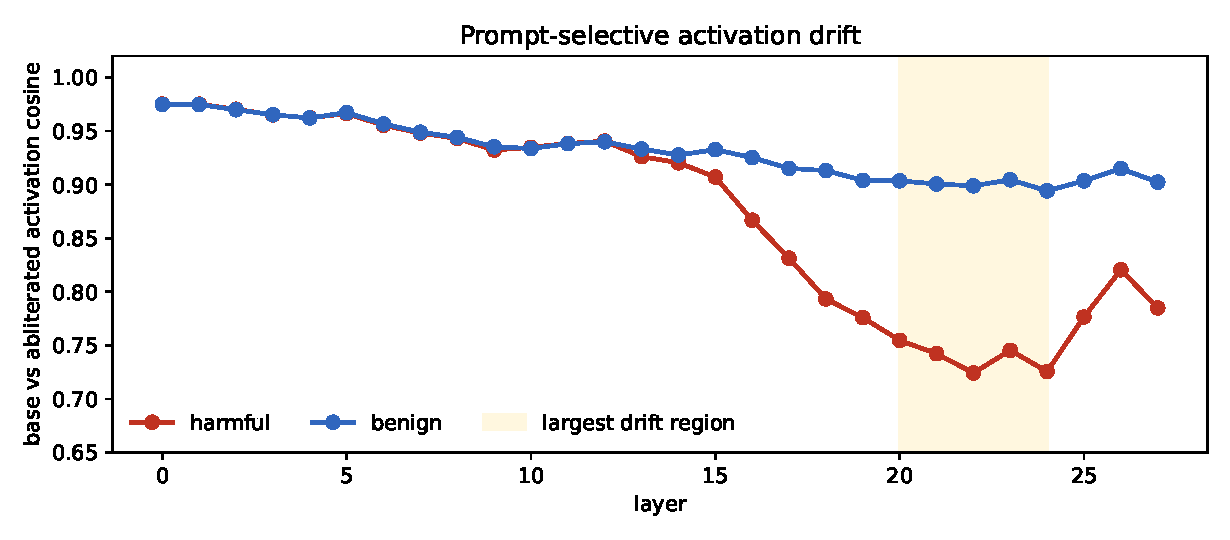
\includegraphics[width=0.84\linewidth]{figures/activation_drift.pdf}
  \end{figure}

  \small
  Harmful prompts drift more than benign prompts in mid-to-late layers; layer 22 is especially different.
\end{frame}

\begin{frame}{Single Modules Were Not Enough}
  Early target-loss patching pointed to mid-layer MLP/block modules.

  \vspace{0.25cm}
  But generation validation failed:
  \begin{itemize}
    \item \texttt{14:mlp}, \texttt{14:block}, \texttt{16:mlp}, and \texttt{16:block} did not restore harmful clean refusal.
    \item This separated likelihood localization from behavioral sufficiency.
  \end{itemize}
\end{frame}

\begin{frame}{RQ3: Broad MLP Range Is Causally Sufficient}
  \begin{figure}
    \centering
    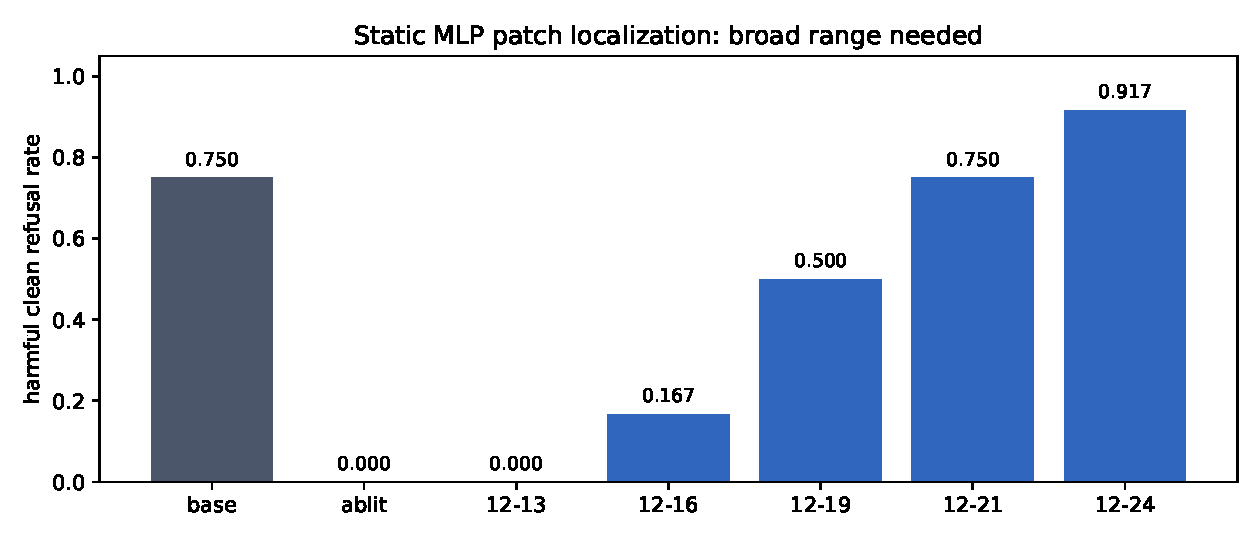
\includegraphics[width=0.86\linewidth]{figures/localization_range.pdf}
  \end{figure}

  \small
  Static base-to-abliterated MLP replacement needs a broad contiguous range. Layers 12-24 repair behavior best.
\end{frame}

\begin{frame}{Activation Patch Confirms Mechanism Level}
  Teacher-forced activation patching over all positions:
  \begin{itemize}
    \item \texttt{12-24:mlp} closes 0.938 of harmful refusal-target loss gap.
    \item \texttt{12-21:mlp} closes 0.937.
    \item \texttt{12-19:mlp} closes 0.917.
  \end{itemize}

  \vspace{0.25cm}
  Target-position-only activation patching closes 0.000 of the gap.

  \vspace{0.25cm}
  Interpretation: the repair is sequence-wide MLP activation propagation, not a single final-token vector.
\end{frame}

\begin{frame}{Generation Patch Confirms Behavior}
  Dynamic activation patching runs the base donor on the current prefix and patches MLP activations into the abliterated recipient during generation.

  \vspace{0.3cm}
  Result on 8 harmful / 8 benign prompts:
  \begin{itemize}
    \item base harmful clean refusal: 0.875.
    \item abliterated harmful clean refusal: 0.000.
    \item dynamic \texttt{12-24:mlp} patch: 1.000.
    \item benign helpfulness remains 1.000; benign over-refusal remains 0.000.
  \end{itemize}
\end{frame}

\section{Current Checkpoint}

\begin{frame}{RQ0: Do Simple Bases Already Explain The Repair?}
  Before SAE/transcoder analysis, we tested compressed baselines:

  \begin{itemize}
    \item mean donor-recipient delta direction per layer;
    \item top changed neurons;
    \item harmful-vs-benign refusal direction;
    \item randomized PCA over activation deltas;
    \item matched random projection controls.
  \end{itemize}

  \vspace{0.25cm}
  This is the key value-action style gate: sparse features must beat honest simpler bases.
\end{frame}

\begin{frame}{Target-Loss Repair: PCA Wins}
  \begin{figure}
    \centering
    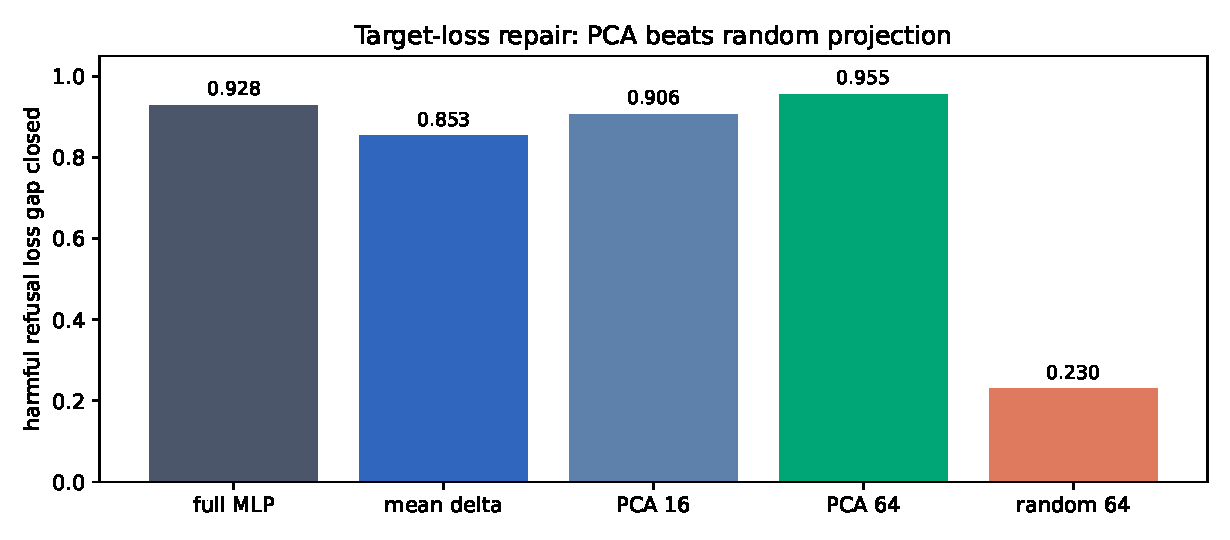
\includegraphics[width=0.86\linewidth]{figures/pca_target_loss.pdf}
  \end{figure}

  \small
  PCA rank 64 closes 0.955 of the harmful refusal-target loss gap. Matched random rank 64 closes only 0.230.
\end{frame}

\begin{frame}{Behavior: Strict Audit Matters}
  \begin{figure}
    \centering
    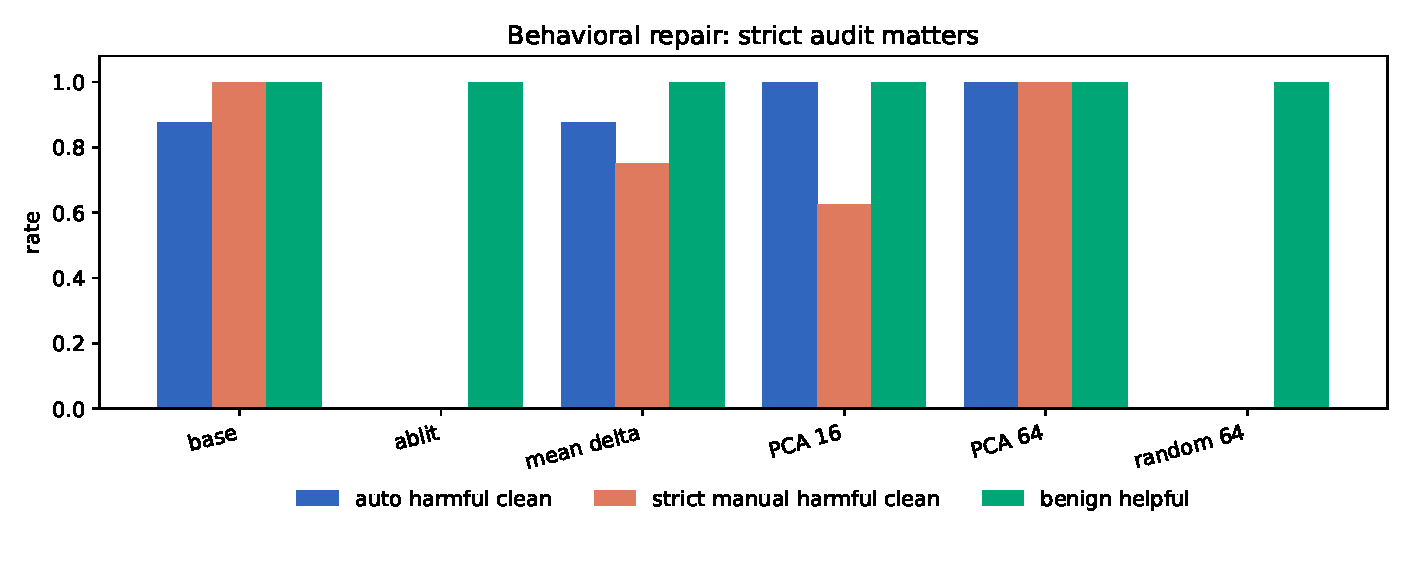
\includegraphics[width=0.92\linewidth]{figures/pca_generation_audit.pdf}
  \end{figure}
\end{frame}

\begin{frame}{Manual Audit Result}
  \begin{table}
    \centering
    \small
    \begin{tabular}{lccc}
      \toprule
      Model or patch & Auto harmful & Strict harmful & Benign helpful \\
      \midrule
      Base & 0.875 & 1.000 & 1.000 \\
      Abliterated & 0.000 & 0.000 & 1.000 \\
      Mean delta rank 1 & 0.875 & 0.750 & 1.000 \\
      PCA rank 16 & 1.000 & 0.625 & 1.000 \\
      PCA rank 64 & 1.000 & 1.000 & 1.000 \\
      Random rank 64 & 0.000 & 0.000 & 1.000 \\
      \bottomrule
    \end{tabular}
  \end{table}

  \vspace{0.15cm}
  \small The automatic scorer over-credited some answers that started with refusal but continued with unsafe advice. PCA rank 64 survived strict manual audit.
\end{frame}

\begin{frame}{Current Mechanistic Interpretation}
  \begin{block}{Best current hypothesis}
    The abliterated TIES merge loses a low-dimensional donor-recipient MLP activation-delta subspace across layers 12-24.
  \end{block}

  \begin{itemize}
    \item Mean-delta rank 1 is a minimal partial repair.
    \item PCA rank 64 is the strongest compressed behavioral repair so far.
    \item Random rank 64 fails, so this is not just any 64-dimensional injection.
    \item SAE/transcoder features must explain, compress, or improve on this PCA subspace.
  \end{itemize}
\end{frame}

\begin{frame}{What Is New Here?}
  The project has moved from ``can we find any model pair?'' to a concrete causal object.

  \begin{itemize}
    \item We have a public model merge that loses a specific behavior.
    \item We can repair it by restoring a broad MLP activation pathway.
    \item We can compress that repair into a low-rank activation-delta subspace.
    \item We discovered a scoring failure mode that matters for safety claims.
  \end{itemize}
\end{frame}

\begin{frame}{What We Should Not Claim Yet}
  \begin{itemize}
    \item Not a proof that model merging is generally safe or unsafe.
    \item Not a full safety benchmark; prompt sets are still small.
    \item Not an SAE result yet.
    \item Not a solved repair mechanism; PCA rank 64 is a strong baseline, not an explanation by itself.
    \item Not a claim that the abliterated merge is useful; it is a failure case we can study.
  \end{itemize}
\end{frame}

\section{Next Steps}

\begin{frame}{Immediate Next Steps}
  \begin{enumerate}
    \item Fix the harmful-refusal evaluator so it detects unsafe continuation after refusal prefixes.
    \item Build held-out harmful and adversarial benign prompt sets.
    \item Revalidate \texttt{pca\_rank64}, mean-delta, full MLP patch, and random controls.
    \item Compare exact or larger-sample PCA to current randomized PCA.
    \item Only then start SAE/transcoder feature experiments.
  \end{enumerate}
\end{frame}

\begin{frame}{What SAE Must Beat}
  A useful sparse feature explanation should show at least one of:

  \begin{itemize}
    \item better repair than PCA rank 64 at similar or lower dimensionality;
    \item interpretable decomposition of the PCA repair into meaningful feature groups;
    \item causal feature patches that recover refusal without unsafe continuation;
    \item prediction of which merges will lose or preserve refusal before generation tests.
  \end{itemize}
\end{frame}

\begin{frame}{Paper Potential}
  \textbf{Current status: continue, do not abandon.}

  \vspace{0.25cm}
  Why:
  \begin{itemize}
    \item real public-model case;
    \item causal repair evidence;
    \item strong non-sparse baseline;
    \item clear evaluation caveat that can become part of the contribution;
    \item natural path to SAE/transcoder comparison.
  \end{itemize}

  \vspace{0.2cm}
  Main risk: if sparse features do not beat PCA or add insight, the paper should be framed as a mechanistic low-rank activation-geometry study rather than an SAE paper.
\end{frame}

\begin{frame}{Artifact Map}
  \small
  \begin{itemize}
    \item Package: \texttt{presentations/2026-05-20-1618-model-merging-full-overview/}
    \item Proposal: \texttt{docs/MECHANISTIC\_MODEL\_MERGING\_SAE\_PROPOSAL.md}
    \item Provenance: \texttt{stage2/results/PROVENANCE.md}
    \item Main Qwen diagnostics: \texttt{stage2/results/qwen1\_5b\_refusal\_rq1\_rq2/}
    \item PCA/random target loss: \texttt{stage2/results/qwen1\_5b\_lowdim\_activation\_patch\_target\_loss\_pca\_random/}
    \item PCA/random generation: \texttt{stage2/results/qwen1\_5b\_lowdim\_activation\_patch\_generation\_pca\_random/}
    \item Manual audit: \texttt{QWEN1\_5B\_LOWDIM\_GENERATION\_MANUAL\_AUDIT.md}
  \end{itemize}
\end{frame}

\begin{frame}{Bottom Line}
  \Large
  We now have a credible model-merging interpretability target:

  \vspace{0.4cm}
  \normalsize
  \begin{center}
    \textbf{A merge-induced refusal failure that can be repaired by restoring a low-rank MLP activation-delta subspace.}
  \end{center}

  \vspace{0.4cm}
  The next decisive question is whether sparse features explain this better than PCA rank 64.
\end{frame}

\end{document}
